\documentclass[11pt]{article}

% Change "review" to "final" to generate the camera-ready version.
\usepackage[preprint]{acl}   % "review" for anonymous submission, "final" for camera-ready

\usepackage{times}
\usepackage{latexsym}
\usepackage[T1]{fontenc}
\usepackage[utf8]{inputenc}
\usepackage{microtype}
\usepackage{inconsolata}
\usepackage{graphicx}
\usepackage{booktabs}
\usepackage{amsmath}
\usepackage{amssymb}
\usepackage{multirow}
\usepackage{url}
\usepackage{colortbl}
\usepackage{tikz}
\usetikzlibrary{arrows.meta, positioning, shapes.geometric, calc, backgrounds, fit}

% ---- shared palette: identical hex values in make_figures.py -------------
\definecolor{jevcyan}{HTML}{00B8D4}
\definecolor{jevelectric}{HTML}{22F0FF}
\definecolor{jevpink}{HTML}{FFAEDC}
\definecolor{jevmagenta}{HTML}{FF2BAF}
\definecolor{jevyellow}{HTML}{FFD84D}
\definecolor{jevink}{HTML}{1A1A2E}
% tints for table cells, so black body text stays legible on top
\definecolor{cellmagenta}{HTML}{FFD6EF}
\definecolor{cellcyan}{HTML}{CFF6FC}
\definecolor{cellyellow}{HTML}{FFF3C4}
\definecolor{cellpink}{HTML}{FFE8F5}
\definecolor{barrest}{HTML}{7FE3F0}
\definecolor{jevgrey}{HTML}{9AA0B4}
\newcommand{\hi}[1]{\cellcolor{cellmagenta}\textbf{#1}}
\newcommand{\hic}[1]{\cellcolor{cellcyan}#1}
\newcommand{\hiy}[1]{\cellcolor{cellyellow}#1}
\newcommand{\hip}[1]{\cellcolor{cellpink}#1}

% ---- inline caption markers, so figures need no in-plot legends ---------
% Built from rules and symbols rather than TikZ: a tikzpicture inside a
% \caption breaks on TikZ's catcode changes.
\newcommand{\mdot}[1]{\textcolor{#1}{\raisebox{0.15ex}{$\bullet$}}}
\newcommand{\msq}[1]{\textcolor{#1}{\rule[0.05ex]{1.05ex}{1.05ex}}}
\newcommand{\mdia}[1]{\textcolor{#1}{\raisebox{0.05ex}{$\blacklozenge$}}}
\newcommand{\mstr}[1]{\textcolor{#1}{\raisebox{-0.1ex}{$\bigstar$}}}
\newcommand{\mbar}[1]{\textcolor{#1}{\rule[-0.25ex]{1.5ex}{1.15ex}}}
\newcommand{\mline}[1]{\textcolor{#1}{\rule[0.45ex]{0.52ex}{0.13ex}\kern0.24ex\rule[0.45ex]{0.52ex}{0.13ex}}}

\title{Certainty Collapses, Calibration Holds: Typed Confidence in a\\Non-Reasoning Decision Model Across Three Mathematics Benchmarks}

\author{
  Adib Sakhawat \\
  Department of Computer Science and Engineering \\
  Islamic University of Technology \\
  Gazipur, Bangladesh \\
  \texttt{sakhadib@gmail.com}
}

\newcommand{\blfootnote}[1]{%
  \begingroup
  \renewcommand\thefootnote{}\footnote{#1}%
  \addtocounter{footnote}{-1}%
  \endgroup
}

\begin{document}
\maketitle

\blfootnote{Code, analysis scripts, aggregated results and the figure sources
are available at \url{https://github.com/sakhadib/JEV_math}. The three
benchmarks and any artifact embedding their text are not redistributed; see
Appendix~\ref{app:repro}.}

\begin{abstract}
A System One model returns a typed decision with a probability distribution in a single forward pass: no chain of thought, no sampling, no text to parse. We evaluate Jev-1.13, the first such model, on 13,110 multiple-choice mathematics items drawn from three benchmarks of increasing difficulty, against three chat models run on identical items under a matched zero-shot direct-choice protocol. Accuracy alone tells a discouraging story: Jev scores 96.94\%, 94.89\% and 54.70\%, is statistically tied with a free stealth model on the two easier benchmarks, and is beaten by 26.6 points on the hardest. Its confidence behaves very differently. As the benchmarks harden, the fraction of items on which Jev commits fully collapses from 53.4\% to 5.2\%, while accuracy on those committed items stays at 100.00\%, 99.79\% and 99.06\%; across all three it answered at maximum confidence 5{,}155 times for 4 errors, of which blind adjudication found 3 to be benchmark key errors rather than model failures. Selective prediction inherits this: deferring the least-confident 10\% of items lifts accuracy to 99.70\% on the easiest benchmark but only to 58.04\% on the hardest, because on hard data there is little confidence to threshold on. We also find that positional bias is not a fixed model property but emerges under uncertainty: Jev's predicted-option marginals match the answer key on both easier benchmarks and diverge sharply on the hardest ($p = 2.3\times10^{-15}$), with the divergence concentrated in low-confidence items and absent in high-confidence ones. We argue that a confidence signal which degrades in step with capability, rather than one that stays high while accuracy falls, is the property worth building on, and that evaluating calibration on benchmarks where every strong system exceeds 94\% cannot detect it.
\end{abstract}

\section{Introduction}

\begin{figure}[t]
\centering
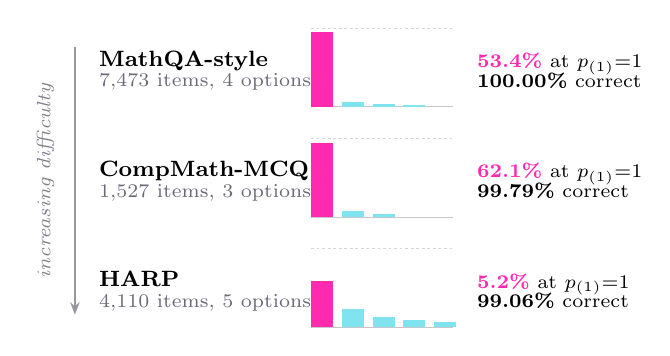
\begin{tikzpicture}[font=\footnotesize, x=1mm, y=1mm]

% ---- difficulty axis
\draw[-{Stealth[length=4.5pt]}, jevink!45, line width=0.7pt]
      (0,3) -- (0,-31);
\node[rotate=90, anchor=south, font=\scriptsize\itshape, text=jevink!55]
      at (-1.4,-14) {increasing difficulty};

% ============================================== row 1
\node[anchor=west, align=left, inner sep=0] at (3,0)
  {\textbf{MathQA-style}\\[-2pt]{\scriptsize\color{jevink!65}7{,}473 items, 4 options}};
\draw[jevink!25, line width=0.4pt] (30,-4.6) -- (48,-4.6);
\draw[jevink!18, line width=0.3pt, dash pattern=on 1pt off 1pt] (30,5.4) -- (48,5.4);
\fill[jevmagenta] (30,-4.6) rectangle (32.8,4.85);
\foreach \i/\p in {1/0.0407, 2/0.0100, 3/0.0038}
  \fill[barrest] (30+\i*3.9,-4.6) rectangle (32.8+\i*3.9,-4.6+\p*10+0.25);
\node[anchor=west, align=left, inner sep=0, font=\scriptsize] at (51,0)
  {{\color{jevmagenta}\textbf{53.4\%}} at $p_{(1)}{=}1$\\[-1pt]\textbf{100.00\%} correct};

% ============================================== row 2
\node[anchor=west, align=left, inner sep=0] at (3,-14)
  {\textbf{CompMath-MCQ}\\[-2pt]{\scriptsize\color{jevink!65}1{,}527 items, 3 options}};
\draw[jevink!25, line width=0.4pt] (30,-18.6) -- (48,-18.6);
\draw[jevink!18, line width=0.3pt, dash pattern=on 1pt off 1pt] (30,-8.6) -- (48,-8.6);
\fill[jevmagenta] (30,-18.6) rectangle (32.8,-9.19);
\foreach \i/\p in {1/0.0472, 2/0.0115}
  \fill[barrest] (30+\i*3.9,-18.6) rectangle (32.8+\i*3.9,-18.6+\p*10+0.25);
\node[anchor=west, align=left, inner sep=0, font=\scriptsize] at (51,-14)
  {{\color{jevmagenta}\textbf{62.1\%}} at $p_{(1)}{=}1$\\[-1pt]\textbf{99.79\%} correct};

% ============================================== row 3
\node[anchor=west, align=left, inner sep=0] at (3,-28)
  {\textbf{HARP}\\[-2pt]{\scriptsize\color{jevink!65}4{,}110 items, 5 options}};
\draw[jevink!25, line width=0.4pt] (30,-32.6) -- (48,-32.6);
\draw[jevink!18, line width=0.3pt, dash pattern=on 1pt off 1pt] (30,-22.6) -- (48,-22.6);
\fill[jevmagenta] (30,-32.6) rectangle (32.8,-26.78);
\foreach \i/\p in {1/0.2031, 2/0.1119, 3/0.0662, 4/0.0369}
  \fill[barrest] (30+\i*3.9,-32.6) rectangle (32.8+\i*3.9,-32.6+\p*10+0.25);
\node[anchor=west, align=left, inner sep=0, font=\scriptsize] at (51,-28)
  {{\color{jevmagenta}\textbf{5.2\%}} at $p_{(1)}{=}1$\\[-1pt]\textbf{99.06\%} correct};

\end{tikzpicture}
\caption{What the model returns, averaged over every item of each benchmark. Bars are the mean probability vector after sorting each item's distribution in descending order, so the leftmost bar (\mbar{jevmagenta}) is the mean probability placed on the model's own answer and the rest (\mbar{barrest}) is the mass it withholds; the dotted rule marks $1.0$. As the benchmarks harden the leading bar shortens and the tail fills in, and the share of items answered at maximum confidence falls from 53.4\% to 5.2\%. Accuracy on those maximally-confident items does not follow it down. The model withdraws certainty rather than misplacing it.}
\label{fig:teaser}
\end{figure}

Large language models answer structured questions by generating unstructured text that a caller then parses. The format may hold or it may not, cost and latency scale with tokens produced, and the confidence, where any is offered, arrives as a sentence rather than a number.

TypeSafe AI's System One class inverts this. A System One model takes an arbitrary text \emph{state} and one or more \emph{typed questions}, and returns typed decisions with probability distributions in a single call. It cannot produce free text, type errors, or out-of-schema values. The first such model, Jev, exposes three question types: \texttt{noul} (a probability), \texttt{choice} (one option plus a distribution over up to 255 caller-defined criteria), and \texttt{score} (a number on a caller-defined scale). There is no chain of thought, no sampling, and no system prompt.

Multi-step arithmetic is the canonical domain where language models benefit from explicit intermediate steps; chain-of-thought prompting \citep{wei2022chain} was demonstrated on exactly this class of problem, and contemporary reasoning models scale test-time compute to push the same benchmarks further \citep{openai2024o1}. A model that cannot reason aloud should therefore be poorly suited to mathematics. Our question is not only whether it is, but whether it knows it is.

Answering that requires difficulty that varies. A single benchmark cannot distinguish a model whose confidence is calibrated from one whose benchmark is easy, and much of the calibration literature operates in a regime where strong systems cluster above 90\%. We therefore run the same protocol over three benchmarks spanning a 42-point accuracy range and ask what happens to the confidence signal as the ground gives way.

Our contributions are:

\begin{enumerate}
\itemsep0em
\item A three-benchmark, four-system evaluation on 13,110 items, with a matched single-judgment protocol and full per-item recording.
\item The central result: Jev's certainty rate collapses by a factor of ten as accuracy falls 42 points, while accuracy conditional on certainty stays above 99\% throughout (Figure~\ref{fig:teaser}).
\item Evidence that positional bias is a property of model $\times$ difficulty rather than of a model, emerging only where the model is uncertain (\S\ref{sec:position}).
\item A blind adjudication of every maximum-confidence error, which finds that 3 of 4 are benchmark key errors, and a resulting proposal to use maximum-confidence disagreement as a benchmark-auditing signal (\S\ref{sec:adjudication}).
\item Evidence that a no-reasoning protocol is unenforceable by prompt and effort setting alone, with billed reasoning tokens as the diagnostic (\S\ref{sec:baselines}).
\end{enumerate}

\section{Related Work}

\paragraph{Reasoning and its absence.}
\citet{wei2022chain} established chain-of-thought prompting as the dominant method for eliciting multi-step reasoning, with arithmetic word problems as the central demonstration. Reasoning models trained to deliberate before answering \citep{openai2024o1} trade latency for accuracy at the far end of that trajectory. \citet{li2025system1to2} survey the landscape through the dual-process lens whose vocabulary we borrow, characterising foundational LLMs as fast System-1-like responders and reasoning LLMs as emulating System-2 deliberation. Jev occupies a position that survey does not cover: a model whose architecture forecloses the System-2 mode rather than one that declines to use it. Our difficulty gradient (\S\ref{sec:difficulty}) makes the cost of that foreclosure measurable.

\paragraph{Mathematics benchmarks.}
\citet{cobbe2021gsm8k} introduced GSM8K and showed that large transformers struggle on multi-step arithmetic without verifier-based reranking, establishing the grade-school word problem as the standard probe. Our three benchmarks span that tradition and move past it: an MathQA-style word-problem set \citep{nlp2025math}, the undergraduate-level CompMath-MCQ \citep{raimondi2026compmath}, and HARP \citep{yue2024harp}, a human-annotated competition set with per-item difficulty levels. The difficulty metadata in the last is what makes the confidence analysis in \S\ref{sec:certainty} possible.

\paragraph{Calibration.}
\citet{guo2017calibration} established that modern deep classifiers are systematically overconfident and introduced the ECE and MCE metrics we report. For language models, \citet{xiong2024can} benchmark verbalized confidence across five models and five task types and again find overconfidence prevailing, with calibration improving as capability increases. \citet{lin2022teaching} show that a model's stated numeric confidence can be a learnable signal distinct from its output distribution, which bears on our finding that Jev returns two different confidence quantities. \citet{yang2024verbalized} add evidence that verbalized confidence reliability is heavily prompt- and architecture-dependent. Against this literature our contribution is not the direction of the gap on any one dataset but its behaviour \emph{across} datasets: the sign flips from underconfident to mildly overconfident as difficulty rises, while conditional reliability at the top of the range holds.

\paragraph{Selective prediction.}
\citet{xin2021abstention} introduced selective prediction to NLP and formalised the accuracy-coverage trade-off we adopt. Our deferral analysis applies that framework to an API-returned distribution rather than to model logits, which is the practically available signal when a model is consumed as a service. We also report where it stops working (\S\ref{sec:selective}), which the framework predicts but which is rarely measured: thresholding cannot manufacture accuracy when little of the mass is confident.

\section{The System One Interface}

\begin{figure*}[t]
\centering
\resizebox{\textwidth}{!}{%
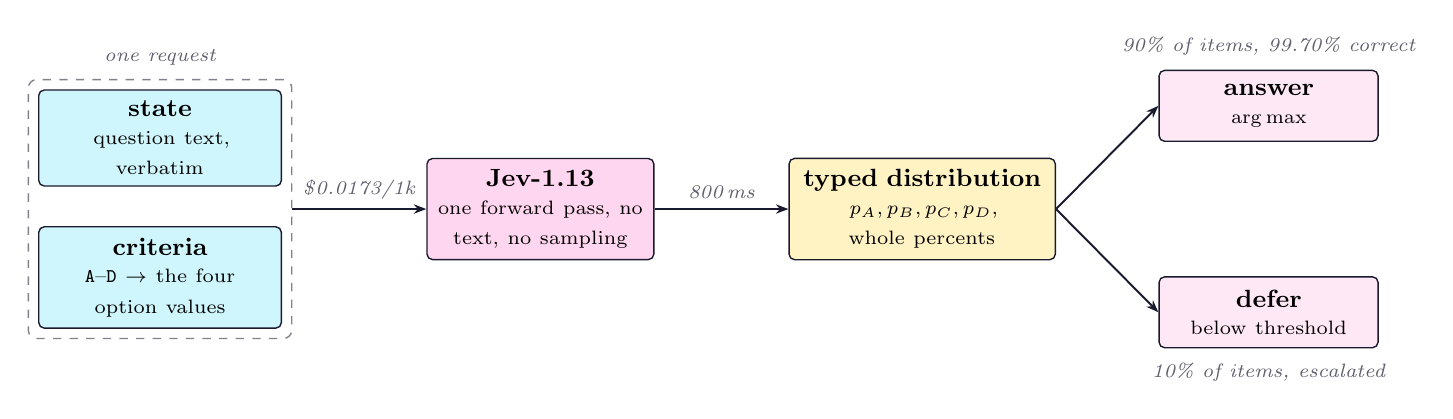
\begin{tikzpicture}[
  font=\small,
  box/.style={rectangle, rounded corners=2pt, draw=jevink, line width=0.5pt,
              align=center, inner sep=4pt, minimum height=9mm},
  lbl/.style={font=\scriptsize\itshape, text=jevink!70},
  ar/.style={-{Stealth[length=4.5pt]}, draw=jevink, line width=0.7pt}
]

\node[box, fill=cellcyan, text width=28mm] (state)
  {\textbf{state}\\[-1pt]{\scriptsize question text, verbatim}};
\node[box, fill=cellcyan, text width=28mm, below=5mm of state] (crit)
  {\textbf{criteria}\\[-1pt]{\scriptsize \texttt{A}--\texttt{D} $\to$ the four option values}};
\node[draw=jevink!55, dashed, line width=0.5pt, rounded corners=3pt,
      fit=(state)(crit), inner sep=3.5pt] (req) {};
\node[lbl, above=0.5mm of req] {one request};

\node[box, fill=cellmagenta, text width=26mm, right=17mm of req] (jev)
  {\textbf{Jev-1.13}\\[-1pt]{\scriptsize one forward pass, no text, no sampling}};

\node[box, fill=cellyellow, text width=31mm, right=17mm of jev] (dist)
  {\textbf{typed distribution}\\[-1pt]{\scriptsize $p_A,p_B,p_C,p_D$, whole percents}};

\node[box, fill=cellpink, text width=25mm, above right=2mm and 13mm of dist] (ans)
  {\textbf{answer}\\[-1pt]{\scriptsize $\arg\max$}};
\node[box, fill=cellpink, text width=25mm, below right=2mm and 13mm of dist] (defer)
  {\textbf{defer}\\[-1pt]{\scriptsize below threshold}};

\draw[ar] (req.east) -- node[lbl, above] {\$0.0173/1k} (jev.west);
\draw[ar] (jev.east) -- node[lbl, above] {800\,ms} (dist.west);
\draw[ar] (dist.east) -- (ans.west);
\draw[ar] (dist.east) -- (defer.west);

\node[lbl, above=0.6mm of ans] {90\% of items, 99.70\% correct};
\node[lbl, below=0.6mm of defer] {10\% of items, escalated};

\end{tikzpicture}}
\caption{The call structure used for every item. The state is the problem text and the four options become \texttt{choice} criteria keyed \texttt{A} to \texttt{D}; one request returns a probability for every key. Because the response is typed, prediction extraction is exact rather than heuristic, and the same response carries the confidence signal that drives the deferral branch on the right. Nothing in this path generates or parses text.}
\label{fig:pipeline}
\end{figure*}

A request carries a \texttt{state} (arbitrary text) and a map of named typed questions. The response carries, for each question, a typed answer with a distribution, plus token usage and cost. For a \texttt{choice} question the caller supplies \texttt{criteria}, a map from keys to descriptions, and the model returns one key together with a probability for every key.

Two properties shape the experiment. There is no output text to parse, so prediction extraction is exact rather than heuristic, and there is no prompt beyond the instruction string attached to the question, so the usual space of prompt-engineering interventions is unavailable.

\section{Experimental Setup}
\label{sec:setup}

\paragraph{Systems.}
\texttt{typesafe/jev-1.13} and three chat models accessed through the same provider: \texttt{openai/gpt-oss-20b}, \texttt{stealth/space-bunny-alpha} (an undocumented endpoint whose identity and parameter count we cannot verify), and \texttt{meta-llama/llama-3.1-8b-instruct}. Every run resolved to a single model build.

\paragraph{Benchmarks.}
Three multiple-choice mathematics sets of increasing difficulty, 13,110 items in total. \textbf{MathQA-style} \citep{nlp2025math}: 7,473 four-option word problems with numeric options. \textbf{CompMath-MCQ} \citep{raimondi2026compmath}: 1,527 three-option undergraduate items in linear algebra, calculus and probability. \textbf{HARP} \citep{yue2024harp}: 4,110 five-option US competition items (AHSME/AJHSME/AMC 8/10/12) carrying per-item difficulty level 1--4, subject, contest and year. None is redistributed here. Because the option count differs across benchmarks (4, 3, 5), the random-guessing floor differs too (25\%, 33.3\%, 20\%), so we treat each benchmark self-contained and read only the \emph{ordering} across them; Appendix~\ref{app:datasets} records the structural properties that make the first two easier than their size suggests.

\paragraph{Protocol.}
For Jev, one call per item: \texttt{state} is the question text verbatim and a single \texttt{choice} question maps the option letters to the stringified option values in the dataset's original order, never shuffled. For the chat models, the question followed by the labelled options and the instruction \emph{``Answer with only the letter of the correct option. Do not explain, do not show any work.''}, at temperature 0 with reasoning effort set to low where supported and a 512-token cap. We score end to end: a reply from which no option can be parsed counts as wrong, because a component that must return a decision has failed to return one.

\paragraph{Tie-breaking.}
Returned probabilities are quantised to whole percents (\S\ref{sec:probs}), so exact ties occur and become common as difficulty rises: 8 items on MathQA-style, 71 on HARP. We re-derive the prediction as the argmax with alphabetical tie-breaking throughout, rather than using the API's undocumented tie-break, which moves the HARP figure by 2 items.

\paragraph{Harness.}
Twelve worker threads paced to at most 15 requests per second, exponential backoff on 429 and 5xx, and an \texttt{fsync} of each completed record as it completes. Every run recorded the complete unmodified API response. All twelve runs (four systems $\times$ three benchmarks) completed every item with zero API errors.

\section{Results}

\subsection{Accuracy across three benchmarks}
\label{sec:accuracy}

\begin{table}[t]
\centering
\small
\setlength{\tabcolsep}{3.4pt}
\begin{tabular}{lrrr}
\toprule
\textbf{System} & \textbf{MathQA} & \textbf{CompMath} & \textbf{HARP} \\
 & \scriptsize 4-opt, 7{,}473 & \scriptsize 3-opt, 1{,}527 & \scriptsize 5-opt, 4{,}110 \\
\midrule
space-bunny & 97.11 & 95.35 & \hi{81.29} \\
gpt-oss-20b & \hi{98.30} & \hi{96.79} & 70.29 \\
Jev-1.13 & 96.94 & 94.89 & 54.70 \\
llama-3.1-8b & 40.09 & 60.12 & 18.32 \\
\midrule
\scriptsize random floor & \scriptsize 25.0 & \scriptsize 33.3 & \scriptsize 20.0 \\
\bottomrule
\end{tabular}
\caption{End-to-end accuracy (\%) on all three benchmarks. Unparseable replies count as wrong. Option counts differ, so the floors differ and cross-benchmark differences are not directly comparable; the ordering is. Wilson intervals and paired tests are in Appendix~\ref{app:baseline}.}
\label{tab:accuracy}
\end{table}

Table~\ref{tab:accuracy} gives the headline. On the two easier benchmarks Jev is statistically tied with space-bunny-alpha (McNemar paired on identical items, $p = 0.51$ and $p = 0.53$) and loses to gpt-oss-20b ($p = 7.5\times10^{-9}$, $p = 0.0013$). On HARP it loses decisively to both ($p = 8.4\times10^{-166}$ and $p = 2.1\times10^{-57}$). No claim that a System One model is better at mathematics than chat models survives this evidence, and we make none.

The two easier benchmarks are also weak instruments. On MathQA-style, 70.6\% of gold values are the smallest of the four options and distractors frequently differ by an order of magnitude, so accuracy partly tracks magnitude plausibility rather than arithmetic. On CompMath-MCQ, 23.5\% of items are number-substituted instances of 117 shared question skeletons, and the items are largely definitional. Appendix~\ref{app:datasets} quantifies both. That gpt-oss-20b, released seven months before CompMath-MCQ was published, scores 96.79\% on it is the cleanest available evidence that the benchmark is intrinsically easy rather than contaminated: a model cannot memorise what did not exist during its training. The corollary is uncomfortable for benchmark design generally. Number-substituted instances of standard textbook questions are re-renderings of material already in every model's training data, so a publication date is not evidence of novelty.

\subsection{The returned distributions}
\label{sec:probs}

Across MathQA-style there are 114 distinct probability values among 29,892 assigned, the smallest non-zero being 0.01: these are percentages, not floats. Sums deviate from 1 by more than $10^{-6}$ on 0.29\% of rows, consistent with independent rounding. Critically for what follows, \textbf{on no item in any benchmark did the model assign zero probability to the gold option}, including every item it answered incorrectly; its distribution never rules out the correct answer.

The API also returns a scalar \texttt{raw.confidence} distinct from the top-1 probability. It disagrees with top-1 on 53.3\% of MathQA-style rows, always downward, and reaches values below what any top-1 probability can attain, so it is a separate and more conservative self-assessment rather than the distribution's maximum. Its mechanism is undocumented. We carry both signals throughout, in the spirit of \citet{lin2022teaching}.

\subsection{Certainty collapses; conditional reliability does not}
\label{sec:certainty}

\begin{table}[t]
\centering
\small
\setlength{\tabcolsep}{3.2pt}
\begin{tabular}{lrrr}
\toprule
 & \textbf{MathQA} & \textbf{CompMath} & \textbf{HARP} \\
\midrule
Overall accuracy & 96.94 & 94.89 & 54.70 \\
Items at $p_{(1)}{=}1$ & 53.4\% & 62.1\% & \hic{5.2\%} \\
\quad count & 3{,}993 & 949 & 213 \\
Accuracy there & \hi{100.00} & \hi{99.79} & \hi{99.06} \\
\midrule
Mean $p_{(1)}$ & 0.9455 & 0.9412 & 0.5817 \\
Conf.\ $-$ accuracy & $-2.4$ & $-0.8$ & $+3.5$ \\
ECE (10 bins) & 0.0239 & 0.0128 & 0.0347 \\
\midrule
Acc.\ at 90\% cov. & 99.70 & 97.82 & \hiy{58.04} \\
\bottomrule
\end{tabular}
\caption{Jev's confidence behaviour as the benchmarks harden. Percentages unless noted. The certainty rate falls tenfold while accuracy conditional on certainty stays above 99\%. The confidence gap flips sign from under- to mildly overconfident, and the value of deferral collapses.}
\label{tab:certainty}
\end{table}

\begin{figure*}[t]
\centering
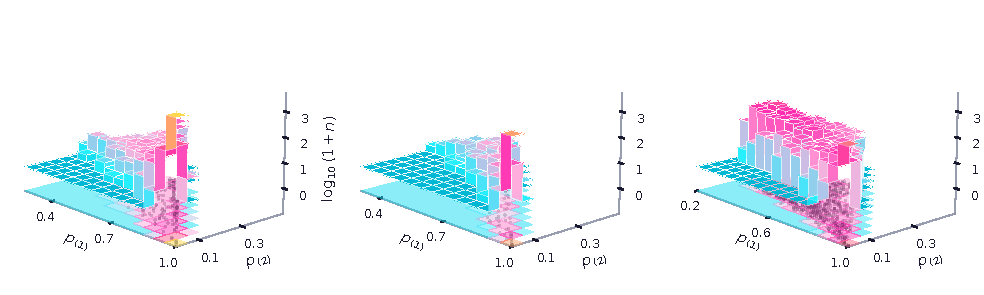
\includegraphics[width=\textwidth]{figures/simplex3.pdf}
\caption{Joint density of the two largest returned probabilities, $p_{(1)}$ and $p_{(2)}$; left to right, MathQA-style, CompMath-MCQ and HARP. Height is $\log_{10}(1+n)$ on a shared scale, surface colour runs low to high as \msq{jevcyan}\,\msq{jevpink}\,\msq{jevmagenta}\,\msq{jevyellow}, the region outside the attainable simplex is masked, and \mdot{jevink} on the floor are errors. The tower at $(1,0)$ on the two easier benchmarks is the model committing fully. On HARP it is gone, replaced by a broad ridge of hedged distributions, and the errors that were confined to the low-$p_{(1)}$ margin now occupy most of the surface.}
\label{fig:simplex3}
\end{figure*}

This is the study's central result, and Table~\ref{tab:certainty} is where it lives. As the benchmarks harden, Jev's accuracy falls 42 points. Over the same range the fraction of items on which it returns a degenerate distribution, placing probability 1 on a single option, falls from 53.4\% to 5.2\%: on HARP it commits fully roughly once in twenty items. Accuracy on those committed items barely moves, from 100.00\% to 99.79\% to 99.06\%.

Figure~\ref{fig:simplex3} shows the same thing in the shape of the distributions. On the easier benchmarks the mass piles into a tower at maximum confidence; on HARP the tower is gone and what remains is a broad ridge of hedged distributions, with errors spread across it rather than confined to its low-confidence margin.

\begin{figure*}[t]
\centering
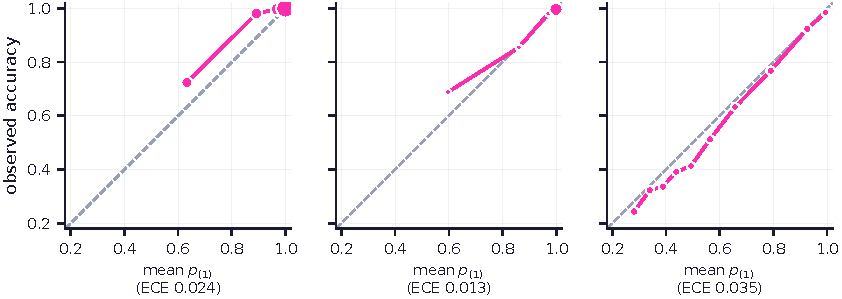
\includegraphics[width=\textwidth]{figures/reliability.pdf}
\caption{Equal-count reliability diagrams on a shared axis, ten bins; left to right, MathQA-style, CompMath-MCQ and HARP. \mdot{jevmagenta} observed accuracy per bin, area proportional to bin count; \mline{jevgrey} perfect calibration. The horizontal extent is itself a result: on the easiest benchmark every bin sits in the top-right corner, and on HARP the bins span the full range because the model rarely asserts much. Points above the diagonal are underconfidence. The easier benchmarks sit above it, HARP tracks it closely and dips below at the top, which is the sign flip recorded in Table~\ref{tab:certainty}.}
\label{fig:reliability}
\end{figure*}

Two secondary movements are worth recording. The confidence gap flips sign: the model is underconfident by 2.4 points on the easiest benchmark and overconfident by 3.5 on the hardest, so the underconfidence we would have reported from a single easy benchmark is not a stable property. Figure~\ref{fig:reliability} shows both movements directly. ECE is also lowest on the middle benchmark, which shows that a single aggregate calibration number is a poor summary of a signal whose behaviour depends on where the task sits relative to the model's capability.

\subsection{Selective prediction, and where it stops working}
\label{sec:selective}

\begin{figure}[t]
\centering
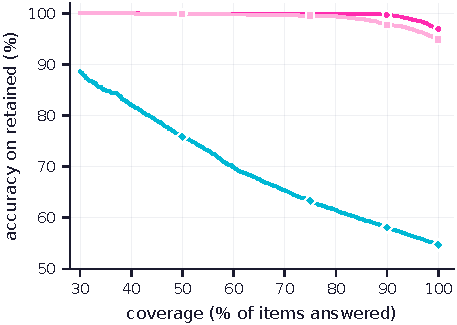
\includegraphics[width=0.97\columnwidth]{figures/coverage3.pdf}
\caption{Accuracy on retained items as coverage falls, thresholding on $p_{(1)}$: \mdot{jevmagenta} MathQA-style, \msq{jevpink} CompMath-MCQ, \mdia{jevcyan} HARP. Deferral is highly effective where confidence is plentiful and nearly powerless where it is not: at 90\% coverage it buys 2.8 points on MathQA-style and 3.3 on HARP, but from 54.7\% rather than 96.9\%.}
\label{fig:coverage3}
\end{figure}

Deferring the least-confident 10\% of items lifts accuracy from 96.94\% to 99.70\% on MathQA-style, from 94.89\% to 97.82\% on CompMath-MCQ, and from 54.70\% to only 58.04\% on HARP (Figure~\ref{fig:coverage3}). The mechanism is visible in Table~\ref{tab:certainty}: thresholding converts confidence into accuracy, and on hard data there is little confidence to convert. Even abstaining on 70\% of HARP leaves accuracy under 89\%.

This is the honest boundary of the deployment argument. A caller can route the 53\% of easy inputs on which the model commits fully and escalate the rest, reaching 99.7\% at 90\% coverage; on competition mathematics the same rule yields a system that is 58\% accurate on the nine items in ten it still answers. The signal remains informative in both regimes, but its cash value depends entirely on where the workload sits.

\subsection{Difficulty gradients separate the categories}
\label{sec:difficulty}

\begin{figure}[t]
\centering
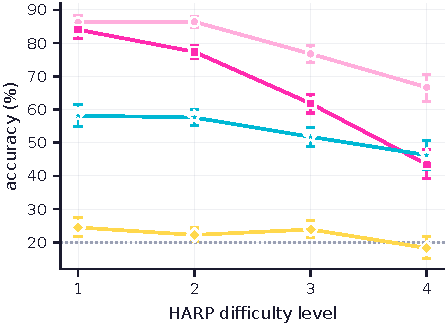
\includegraphics[width=0.97\columnwidth]{figures/difficulty.pdf}
\caption{HARP accuracy by annotated difficulty level, with Wilson 95\% intervals: \mdot{jevpink} space-bunny-alpha, \msq{jevmagenta} gpt-oss-20b, \mstr{jevcyan} Jev-1.13, \mdia{jevyellow} llama-3.1-8b. The dotted rule is the 20\% five-option floor. The single-pass systems are flat and low; the reasoning systems start high and fall. gpt-oss-20b's gradient is steepest, and by level 4 it no longer separates from Jev.}
\label{fig:difficulty}
\end{figure}

HARP's per-item difficulty levels let us see the gradient directly (Figure~\ref{fig:difficulty}). Jev declines gently, 58.2\% to 46.2\% across levels 1 to 4, and llama-3.1-8b is flat near chance throughout. The reasoning-capable systems decline steeply from a much higher start: gpt-oss-20b falls 84.0\% to 43.5\%, space-bunny-alpha 86.2\% to 66.7\%.

The crossing is the notable part. gpt-oss-20b leads Jev by 15.6 points overall but by level 4 its advantage has vanished, 43.5\% against Jev's 46.2\% (overlapping intervals; we claim convergence, not a reversal). Hidden deliberation buys a great deal on levels 1--2 and nothing at level 4. Only space-bunny-alpha sustains an advantage at the top of the difficulty range. By subject, Jev is weakest on number theory (39.7\%) and strongest on prealgebra (62.9\%).

\subsection{Positional bias emerges under uncertainty}
\label{sec:position}

\begin{figure*}[t]
\centering
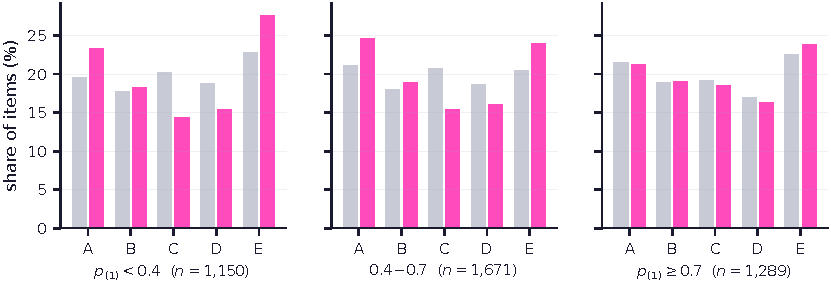
\includegraphics[width=\textwidth]{figures/position.pdf}
\caption{Option marginals on HARP, split by confidence band (left to right: $p_{(1)}<0.4$, $0.4$ to $0.7$, $p_{(1)}\geq0.7$). \mbar{jevgrey} share of items whose key is that letter, \mbar{jevmagenta} share Jev predicts. Where the model is uncertain it over-selects the first and last options and avoids the middle; where it is confident its marginals track the key. Positional bias is a property of model $\times$ difficulty, not of the model.}
\label{fig:position}
\end{figure*}

On both easier benchmarks Jev's predicted option marginals are indistinguishable from the answer key ($\chi^2(3)$, $p = 0.960$ and $p = 0.837$), which in a single-benchmark study would support a clean bill of health. On HARP the same test gives $p = 2.3\times10^{-15}$. The model over-predicts A ($+99$ items) and E ($+130$) and under-predicts C ($-162$) and D ($-90$), and per-gold-letter accuracy spreads 7.7 points, from 58.8\% when the answer is A to 51.1\% when it is C.

Figure~\ref{fig:position} localises it. Splitting by confidence, the divergence is concentrated where the model is uncertain, and at $p_{(1)} \geq 0.7$ the predicted marginals track the key closely. The model is not positionally biased; it falls back on an edge-position heuristic when it does not know, which is a different and more specific claim. The methodological consequence is that a position-bias null measured on a benchmark a model finds easy carries no information about its behaviour on a harder one, and the three-consecutive-benchmark null we would have reported for llama-3.1-8b, which is severely biased everywhere, is not the same kind of evidence as Jev's.

\subsection{Adjudicating maximum-confidence errors}
\label{sec:adjudication}

Across 13,110 items Jev returned a degenerate distribution 5,155 times and was scored wrong on 4 of them. Because that number is small enough to inspect and consequential enough to matter, we adjudicated all four by hand against the source mathematics.

Three are benchmark key errors. On a CompMath-MCQ item asking for the variance of a Gaussian with density proportional to $\exp\{-(x-3)^2/8\}$, matching $\exp\{-(x-\mu)^2/2\sigma^2\}$ gives $\sigma^2 = 4$, which is what Jev answered; the key records 2, which is $\sigma$. On a second, asking which NumPy function takes a separate array of weights, Jev answered \texttt{np.average}, which has a \texttt{weights} argument; the key records \texttt{np.mean}, which does not. On a HARP geometry item asking for $P/K$ for a triangle circumscribing a circle of radius $r$, the incircle identity $K = rP/2$ gives $2/r$, which is what Jev answered and also what both other answering systems answered; the key records $2/\sqrt{r}$.

One is a genuine model error: on a HARP item about right-to-left operator grouping, the correct reading of $a \div b - c + d$ is $a/(b-c-d)$ and Jev returned $a/(b-c+d)$, a sign error.

The corrected record is 5,154 of 5,155, an error rate of 0.019\% with an exact binomial 95\% interval of $[0.0005\%, 0.108\%]$. We report the as-scored figures in Table~\ref{tab:certainty} and elsewhere, since accepting the adjudication requires accepting our mathematics; the adjudicated figure is the one we believe. Either way the conclusion is the same, and a second observation follows from it. If maximum-confidence disagreement with a key is more often a key error than a model error, it is a cheap auditing signal for benchmark quality: 4 items to check across 13,110, yielding 3 corrections. The 266 HARP items that all four systems miss are the natural next place to look, and one of them is the geometry item above.

\subsection{Chat-model baselines and protocol compliance}
\label{sec:baselines}

Two properties separate the systems independently of accuracy. First, Jev returned a parseable decision on every one of 13,110 items by construction, against 7 to 867 failures per chat model per benchmark, almost all of them empty replies that exhausted the token budget. Second, no chat model exposes a per-option confidence under this protocol, so none can be placed on the curves of Figure~\ref{fig:coverage3} at all.

The no-reasoning protocol also did not hold. gpt-oss-20b was billed for reasoning tokens on 93.1\% of MathQA-style items and 93.5\% of HARP items, despite both the effort setting and the explicit instruction, with a mean of 274 tokens per item on HARP. Its visible output was a bare letter; the accuracy behind it was bought with hidden chain of thought, and its 863 empty HARP replies are items where it spent the whole budget thinking. space-bunny-alpha reports zero reasoning tokens yet produced 488 truncation-empties, which is the signature of unbilled internal generation. A no-reasoning protocol cannot be enforced on a reasoning-capable model through prompt wording and an effort parameter; billed reasoning tokens are a partial diagnostic and unbilled deliberation is not observable at all.

\subsection{Cost and latency}
\label{sec:cost}

Jev's latency is flat at a median of 794, 793 and 793\,ms across the three benchmarks despite LaTeX-formatted input in two of them, is uncorrelated with input length ($r = -0.015$, $p = 0.19$), and does not differ between correct and incorrect answers (Mann-Whitney, $p = 0.97$): the model does not take longer when it is about to be wrong, which is the behaviour the framing predicts and the opposite of what test-time-compute models are designed to do \citep{openai2024o1}. It was also the fastest system on every benchmark, completing HARP in 428\,s against 3{,}482\,s for gpt-oss-20b and 4{,}552\,s for space-bunny-alpha, at \$0.083. Billing reconciles exactly against published per-token pricing. Full figures are in Appendix~\ref{app:cost}.

\section{Discussion}
\label{sec:discussion}

The accuracy story is quickly told and mostly negative. A model that cannot reason aloud is competitive on benchmarks that do not require reasoning and is not competitive on one that does. On HARP it trails a stealth frontier model by 26.6 points, and the 54.70\% it does reach rests on a five-option format where the floor is 20\%.

What survives is a claim about the confidence signal, and the three-benchmark design is what licenses it. A calibration result from any one of these benchmarks would have been misleading in a specific way. MathQA-style alone would have supported "never confidently wrong" and a 2.4-point underconfidence gap. CompMath-MCQ alone would have supported a near-zero gap and the best ECE of the three. HARP alone would have shown mild overconfidence and a deferral curve barely worth drawing. Only together do they show the thing that is actually stable: the model withdraws certainty as the task outruns it, by a factor of ten, while what it still asserts at maximum confidence stays reliable to within one item in five thousand.

That is a property worth naming, because the failure mode it excludes is the one that matters operationally. A component whose confidence stays high while its accuracy falls is worse than useless in a routing system, since it fails silently and at scale. Jev's confidence falls faster than its accuracy does. The cost is that deferral stops buying much on hard workloads (\S\ref{sec:selective}), and a caller should read Figure~\ref{fig:coverage3} as a statement about their own data rather than about the model.

Two findings generalise past this model. Positional bias measured on an easy benchmark tells you nothing about a hard one (\S\ref{sec:position}); it is a fallback behaviour that surfaces under uncertainty, so the standard practice of reporting a single $\chi^2$ null is underpowered by construction. And maximum-confidence disagreement with an answer key is a usable benchmark-auditing signal (\S\ref{sec:adjudication}), which in our case was right three times out of four.

\section{Conclusion}

A model that cannot reason aloud answered 13,110 mathematics items as single sub-second judgments. Its accuracy ranged from 96.94\% on easy word problems to 54.70\% on competition mathematics, where a stealth frontier model reached 81.29\%. On raw capability the result is unremarkable and, at the hard end, poor.

The confidence signal is a different matter. Across a 42-point accuracy range the model's certainty rate fell by a factor of ten while its accuracy when certain stayed above 99\%, and across all three benchmarks it committed fully 5,155 times for a single genuine error. Positional bias appeared only where confidence was absent, and three of the four maximum-confidence errors turned out to be mistakes in the benchmarks rather than in the model. We would not have learned any of this from one benchmark, and we would have drawn three different and individually plausible wrong conclusions from each of them alone.

\section{Limitations}
\label{sec:limitations}

\paragraph{Contamination cannot be ruled out and varies by benchmark.}
All three benchmarks predate or may predate the training cutoffs of the systems we measure, and competition mathematics in particular is heavily reproduced online. We can say that CompMath-MCQ is intrinsically easy rather than merely memorised, because gpt-oss-20b predates it by seven months and still scores 96.79\% (\S\ref{sec:accuracy}); we cannot say the same for Jev, whose training data is undisclosed, and we can say nothing either way about HARP. Differential contamination between systems is not testable from our data and would shift the comparisons in an unknown direction.

\paragraph{The baseline is narrow.}
Three models, one prompt, one decoding configuration, one run each, and no frontier chat model. One of the three did not honour the no-reasoning protocol and a second appears not to have either (\S\ref{sec:baselines}), so the matched single-judgment comparison rests on shakier ground than the table suggests, and one of the two remaining models is an undocumented endpoint whose identity, size and training we cannot verify. A reasoning model given explicit permission to reason would likely exceed every accuracy reported here; we did not measure that ceiling.

\paragraph{Option counts differ across benchmarks.}
Four, three and five options give floors of 25\%, 33.3\% and 20\%, and change the shape of the attainable simplex. Cross-benchmark accuracy differences are therefore not clean measurements of difficulty, and part of the rise in the certainty rate from MathQA-style to CompMath-MCQ is attributable to mass concentrating more easily over three options than four. We read only the ordering across benchmarks, never the magnitudes.

\paragraph{Template structure inflates effective sample size.}
23.5\% of CompMath-MCQ items are number-substituted instances of shared skeletons, with one family appearing 18 times. Wilson intervals assume independent items, so the intervals we report for that benchmark are too narrow. A cluster bootstrap over skeletons would correct this; we did not run one.

\paragraph{The adjudication is ours.}
Four maximum-confidence errors were adjudicated by one author against the source mathematics (\S\ref{sec:adjudication}). Three of the four are arithmetic or API facts rather than judgment calls, and on the geometry item two independent systems agree with our reading, but no blind second annotator was used. We report as-scored figures throughout so that no headline depends on accepting it.

\paragraph{Quantised probabilities, and ties that scale with difficulty.}
Resolution below one percentage point does not exist. Exact ties rise from 8 items on MathQA-style to 71 on HARP as the distribution flattens, so the tie-breaking rule becomes materially more load-bearing exactly where the model is least certain.

\paragraph{One prompt, one ordering, one run.}
No seed variation, so run-to-run variance is unmeasured; the API exposes no sampling controls, so it may be zero, but that is an assumption. Option order was never shuffled, which matters more given \S\ref{sec:position}: we measure bias under one fixed ordering.

\paragraph{API artifacts are not model internals.}
The \texttt{raw.confidence} scalar, billed reasoning-token counts, and the undocumented tie-break are properties of served APIs. Unbilled deliberation is invisible to us, which limits what we can conclude about space-bunny-alpha in particular.

\section{Future Work}
\label{sec:future}

In descending order of how much they would change our reading: (1) a free-form variant with no options, to separate solving from elimination on the two easier benchmarks; (2) a broader baseline including frontier chat models and a reasoning model permitted to reason, to establish the ceiling HARP admits; (3) a shuffled-order rerun of HARP, to test whether the edge-position fallback of \S\ref{sec:position} follows the positions or the content; (4) blind two-annotator adjudication of the 266 items all four systems miss, to estimate HARP's key-error rate and test the auditing proposal of \S\ref{sec:adjudication}; (5) a repeat run to establish determinism, particularly on the 71 tied HARP items; and (6) a probe set designed to make the two confidence signals diverge, to characterise \texttt{raw.confidence} mechanically.

\bibliography{custom}

\appendix

\section{Protocol Details}
\label{app:protocol}

\paragraph{Jev request.} Three fields: the model identifier; \texttt{state} set to the question string verbatim, with no wrapper or embedded instruction; and \texttt{questions} containing one entry of type \texttt{choice}, whose instruction string is quoted in \S\ref{sec:setup} and whose \texttt{criteria} map option letters to the stringified option values in the dataset's original order. Letters rather than values are used as keys because option values can collide within an item.

\paragraph{Chat request.} The question text, a blank line, \texttt{Options:} and the labelled options one per line, then the instruction quoted in \S\ref{sec:setup}. HARP runs additionally appended an explicit prohibition on reasoning, which did not change the behaviour reported in \S\ref{sec:baselines}.

\paragraph{Parsing.} A chat reply counts as parsed when a single option letter can be recovered. HARP runs used an extended parser accepting \texttt{ANSWER:} tags and boxed answers in addition to a lone letter; the two easier benchmarks used lone-letter parsing only. This makes parse-failure counts not strictly comparable across benchmarks, though in every run the unrecoverable failures were empty strings, which no parser recovers.

\paragraph{Recording.} Per item we store the resolved model build, response identifier, UTC timestamp, the returned choice and full distribution, the API confidence scalar, token counts including billed reasoning tokens, cost, client-measured latency, attempt count, and the unmodified response object.

\section{Benchmark Properties}
\label{app:datasets}

\paragraph{MathQA-style.} All 7,473 gold values are integers. In 5,276 items (70.6\%) the gold is the smallest of four options and in 946 (12.7\%) the largest; median option spread ($\max/\min$) is near 25. Accuracy tracks this structure: 98.5\% when the gold is smallest against 91.2\% when it is neither smallest nor largest, and 98.7\% on the widest option-spread quartile against 93.8\% on the tightest. An unknown share of accuracy on this benchmark is magnitude plausibility rather than arithmetic. Internal near-duplication is negligible: zero exact duplicates and one near-duplicate pair at shingle-Jaccard $\geq 0.6$.

\paragraph{CompMath-MCQ.} Normalising digits collapses 1,527 questions to 1,285 skeletons; 359 items (23.5\%) share a skeleton with at least one other, the largest family appearing 18 times. For the three strong systems, template-family items are only 1--2 points easier than unique items, so the benchmark's ease is intrinsic rather than driven by repetition. For llama-3.1-8b the sign reverses (51.5\% on template items against 62.8\% on unique ones), because the largest family covers a concept it consistently gets wrong.

\paragraph{HARP.} 4,110 items with difficulty level 1--4 ($n = 858$, 1{,}612, 1{,}136, 504), six subjects, and contest and year metadata. 266 items (6.5\%) are missed by all four systems; at least one is a key error (\S\ref{sec:adjudication}).

\section{Full Baseline Results}
\label{app:baseline}

\begin{table}[h]
\centering
\small
\setlength{\tabcolsep}{3pt}
\begin{tabular}{llrrr}
\toprule
\textbf{Bench.} & \textbf{System} & \textbf{Acc.} & \textbf{No ans.} & \textbf{McNemar} \\
\midrule
\multirow{4}{*}{MathQA}
 & gpt-oss & 98.30 & 95 & $7.5\!\times\!10^{-9}$ \\
 & space-bunny & 97.11 & 43 & 0.51 \\
 & Jev & 96.94 & \hic{0} & --- \\
 & llama-8b & 40.09 & 7 & $<\!10^{-300}$ \\
\midrule
\multirow{4}{*}{CompMath}
 & gpt-oss & 96.79 & 3 & 0.0013 \\
 & space-bunny & 95.35 & 11 & 0.53 \\
 & Jev & 94.89 & \hic{0} & --- \\
 & llama-8b & 60.12 & 64 & $1.6\!\times\!10^{-126}$ \\
\midrule
\multirow{4}{*}{HARP}
 & space-bunny & 81.29 & 490 & $8.4\!\times\!10^{-166}$ \\
 & gpt-oss & 70.29 & 867 & $2.1\!\times\!10^{-57}$ \\
 & Jev & 54.70 & \hic{0} & --- \\
 & llama-8b & 18.32 & 538 & $1.4\!\times\!10^{-268}$ \\
\bottomrule
\end{tabular}
\caption{End-to-end accuracy (\%), count of items with no parseable answer, and McNemar exact test against Jev on paired items. On HARP, accuracy computed only over items a system actually answered is 92.3\% for space-bunny-alpha and 89.1\% for gpt-oss-20b; llama-3.1-8b's 18.32\% rises to 22.65\% under extended parsing, which recovers verbose but decisive replies.}
\end{table}

\paragraph{Position bias in the baselines.} llama-3.1-8b is severely biased on all three benchmarks ($\chi^2$ $p \approx 0$ throughout; 46.8\% of its HARP answers are option A), which is why its accuracy overstates its competence. gpt-oss-20b and space-bunny-alpha are clean on all three. Jev is clean on the two easier benchmarks and biased on HARP (\S\ref{sec:position}).

\section{Cost, Latency and Throughput}
\label{app:cost}

\begin{table}[h]
\centering
\small
\setlength{\tabcolsep}{3.5pt}
\begin{tabular}{llrrr}
\toprule
\textbf{Bench.} & \textbf{System} & \textbf{p50 lat.} & \textbf{Wall} & \textbf{Cost} \\
\midrule
\multirow{4}{*}{MathQA}
 & Jev & \hic{794\,ms} & \hic{499\,s} & \$0.130 \\
 & llama-8b & 1{,}155\,ms & 859\,s & \$0.022 \\
 & gpt-oss & 1{,}817\,ms & 2{,}859\,s & \$0.140 \\
 & space-bunny & 1{,}427\,ms & 3{,}881\,s & free \\
\midrule
\multirow{4}{*}{CompMath}
 & Jev & \hic{793\,ms} & \hic{297\,s} & \$0.025 \\
 & llama-8b & 1{,}147\,ms & 463\,s & \$0.005 \\
 & gpt-oss & 1{,}536\,ms & 1{,}069\,s & \$0.025 \\
 & space-bunny & 1{,}395\,ms & 1{,}292\,s & free \\
\midrule
\multirow{4}{*}{HARP}
 & Jev & \hic{793\,ms} & \hic{428\,s} & \$0.083 \\
 & llama-8b & 923\,ms & 916\,s & \$0.030 \\
 & gpt-oss & 4{,}050\,ms & 3{,}482\,s & \$0.210 \\
 & space-bunny & 2{,}103\,ms & 4{,}552\,s & free \\
\bottomrule
\end{tabular}
\caption{Median per-item latency, wall-clock for the full run, and total cost. Jev's median latency is flat to within 1\,ms across three benchmarks with different input formats. Wall-clock is not a clean capability comparison: the free endpoint is presumably throttled and Jev's runs sat on our own 15\,req/s pacing cap.}
\end{table}

Jev's output-token count is a constant 45 on every item with no generated text, which is a billing envelope for the typed response rather than content; output is priced at zero, so it has no cost consequence. On MathQA-style, summed per-call cost of \$0.129608 equals the expected cost at the published \$0.042 per million input tokens to the last reported digit.

\section{Additional Figures}
\label{app:extra}

\begin{figure}[h]
\centering
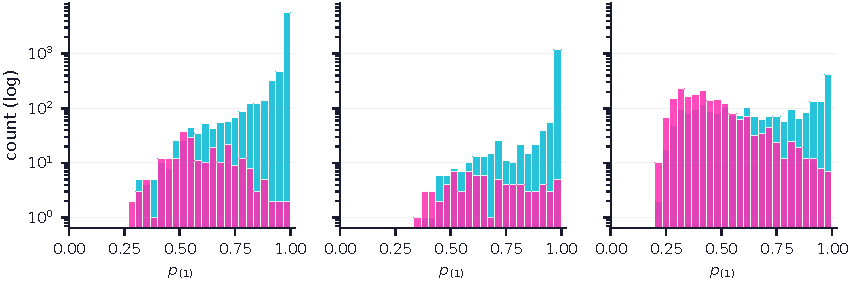
\includegraphics[width=0.97\columnwidth]{figures/confidence.pdf}
\caption{Top-1 probability by outcome, log count; left to right, MathQA-style, CompMath-MCQ and HARP. \mbar{jevcyan} correct, \mbar{jevmagenta} incorrect. On the easier benchmarks errors sit in the middle of the range and vanish at the top. On HARP the correct and incorrect distributions overlap heavily, which is the distributional form of the deferral collapse in \S\ref{sec:selective}.}
\label{fig:confhist}
\end{figure}

\section{Reproduction}
\label{app:repro}

This appendix states what is needed to repeat the study independently of our code.

\paragraph{Calls.} For the typed model, post the question text as \texttt{state} with a single \texttt{choice} question whose criteria map option letters to stringified option values in the dataset's original order. For chat baselines, present question, options and a letter-only instruction at temperature 0 with a low reasoning-effort setting and a 512-token cap. Record the full response object in both cases, including billed reasoning tokens, which are the only visible evidence that a model reasoned despite instruction.

\paragraph{Scoring.} Score end to end, counting unparseable or empty replies as wrong. Re-derive the typed model's prediction as an argmax with a fixed tie-breaking rule rather than trusting an undocumented one; ties become common on hard benchmarks once probabilities are quantised. Compare systems with McNemar exact tests paired over items, not by comparing marginal accuracies.

\paragraph{Analysis parameters.} Wilson intervals for proportions; exact binomial intervals for near-zero error rates; calibration under both equal-count and equal-width binning with ten bins; 2,000 bootstrap resamples; NLL with clipping $\epsilon = 10^{-3}$, which is nearly inconsequential because no gold option ever receives zero probability.

\paragraph{One numerical trap.} When binning returned probabilities, construct histogram edges so the final edge lies strictly above 1.0. Edges accumulated from a floating-point step can terminate just below it and silently discard every item whose top probability is exactly 1.0, which on the easiest benchmark is over half the data and precisely the subset carrying the central result.

\paragraph{Environment.} Python 3.12.3, numpy 2.5.3, pandas 3.0.6, matplotlib 3.11.2, scipy 1.18.1. Seeds: 42 for qualitative sampling, 20260928 for bootstrap.

\paragraph{Availability.} Run and analysis code, aggregated tables behind every number reported here, and figure sources are released. The three benchmarks and any artifact embedding their text, including per-item results, are withheld under their respective terms.

\end{document}
